%
% SchedWeek.tex
% Weekly Recurring Events Schedule
%
% Aleph Objects Operations Manual
%
% Copyright (C) 2014, 2015 Aleph Objects, Inc.
%
% This document is licensed under the Creative Commons Attribution 4.0
% International Public License (CC BY-SA 4.0) by Aleph Objects, Inc.
%

% To extract just the schedule pages from the PDF, run something like:
% pdfjoin AOOM.pdf 37 -o AOOM-schedule.pdf

% These set the width of a day and the height of an hour.
\newcommand*\daywidth{3.7cm}
\newcommand*\hourheight{3.8em}

% The entry style will have two options:
% * the first option sets how many hours the entry will be (i.e. its height);
% * the second option sets how many overlapping entries there are (thus
%   determining the width).
\tikzset{entry/.style 2 args={
    xshift=(0.5334em+0.8pt)/2,
    draw,
    line width=0.8pt,
    font=\sffamily,
    rectangle,
    rounded corners,
    fill=blue!20,
    anchor=north west,
    inner sep=0.3333em,
    text width={\daywidth/#2-1.2em-1.6pt},
    minimum height=#1*\hourheight,
    align=center
}}

% Start the picture and set the x coordinate to correspond to days and the y
% coordinate to correspond to hours (y should point downwards).
\begin{sidewaysfigure}[p]
\thisfloatpagestyle{empty}
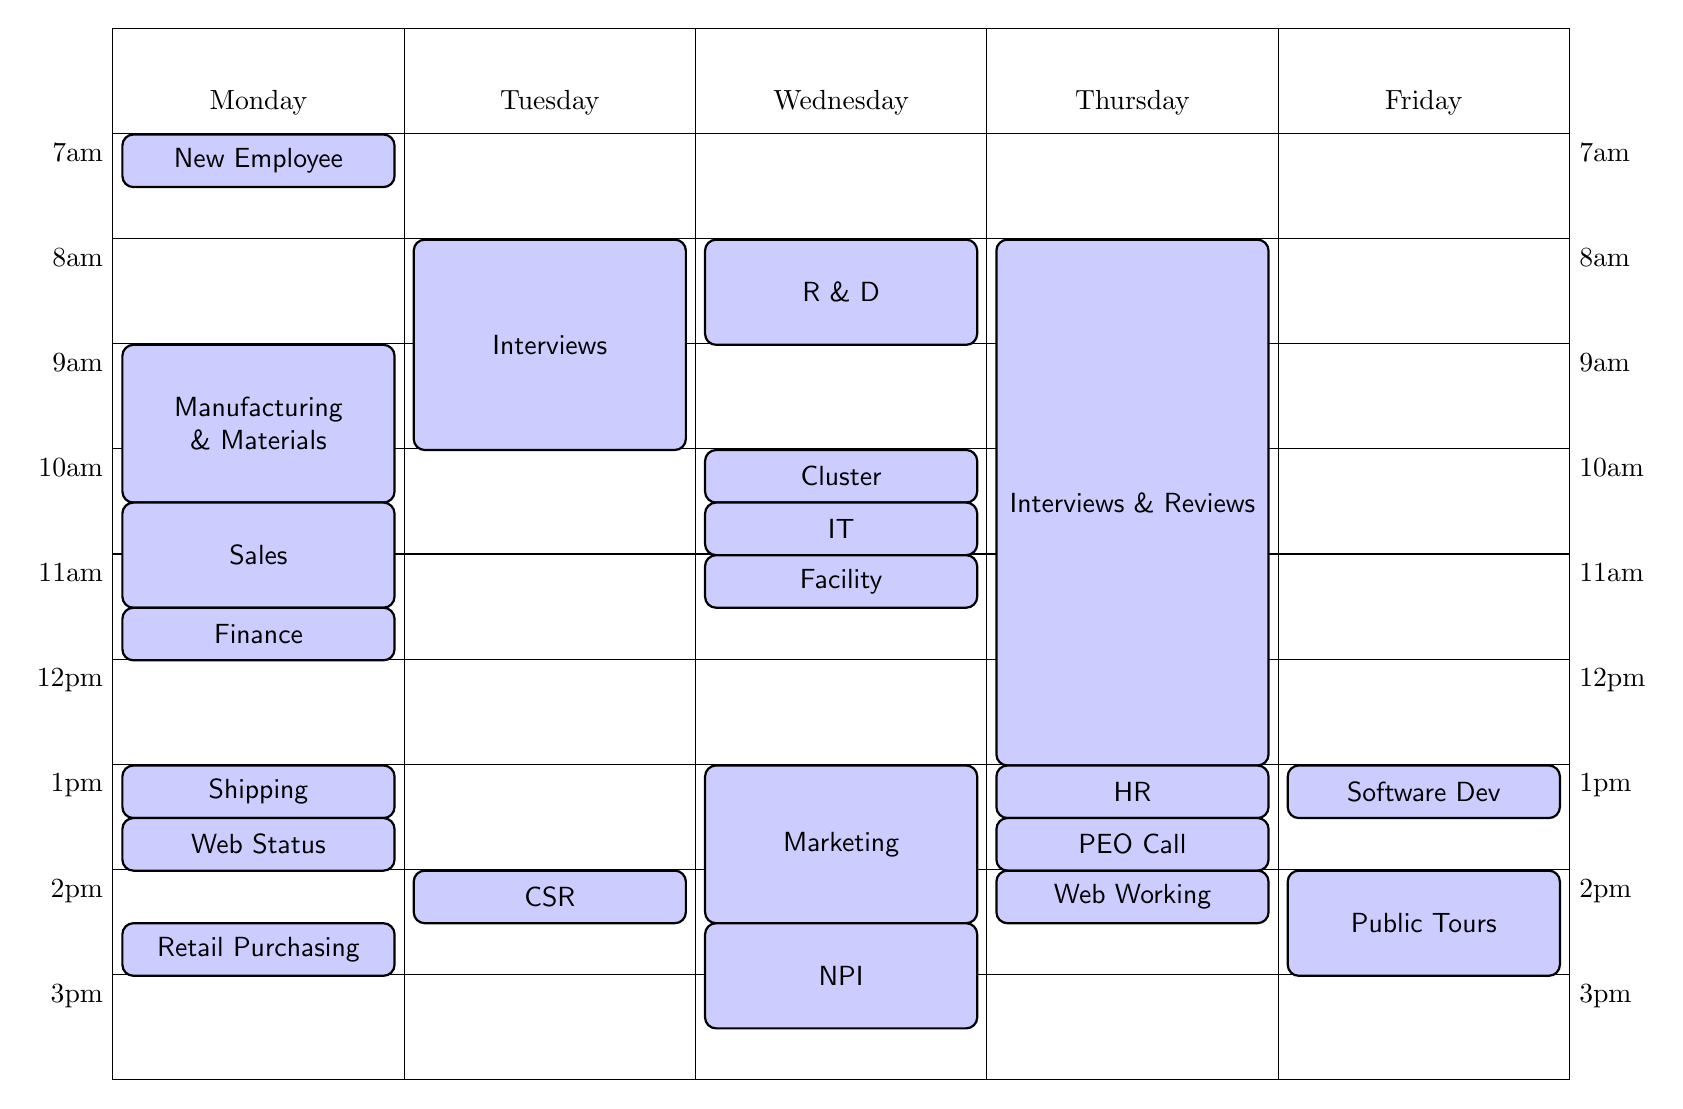
\begin{tikzpicture}[y=-\hourheight,x=\daywidth]

    % First print a list of times.
    \foreach \time/\ustime in {7/7am,8/8am,9/9am,10/10am,11/11am,12/12pm,13/1pm,14/2pm,15/3pm}
        \node[anchor=north east] at (1,\time) {\ustime};

    % Draw some day dividers.
    \draw (1,6) -- (1,16);
    \draw (2,6) -- (2,16);
    \draw (3,6) -- (3,16);
    \draw (4,6) -- (4,16);
    \draw (5,6) -- (5,16);
    \draw (6,6) -- (6,16);
    
    % Draw some hour dividers.
    \draw (1,6) -- (6,6);
    \draw (1,7) -- (6,7);
    \draw (1,8) -- (6,8);
    \draw (1,9) -- (6,9);
    \draw (1,10) -- (6,10);
    \draw (1,11) -- (6,11);
    \draw (1,12) -- (6,12);
    \draw (1,13) -- (6,13);
    \draw (1,14) -- (6,14);
    \draw (1,15) -- (6,15);
    \draw (1,16) -- (6,16);

    \foreach \time/\ustime in {7/7am,8/8am,9/9am,10/10am,11/11am,12/12pm,13/1pm,14/2pm,15/3pm}
        \node[anchor=north west] at (6,\time) {\ustime};
        
    % Start Monday.
    % Write the entries. Note that the x coordinate is 1 (for Monday) plus an
    % appropriate amount of shifting. The y coordinate is simply the starting
    % time.
    % 1=Monday, 2=Tuesday, 3=Wednesday, 4=Thursday, 5=Friday
    %\node[entry={DURATION}{COLUMN WIDTH?}] at (DAY,HOUR) {TEXT};
    \node[anchor=north] at (1.5,6.5) {Monday};
    \node[entry={0.5}{1}] at (1,7) {New Employee};
    \node[entry={1.5}{1}] at (1,9) {Manufacturing \& Materials};
    \node[entry={1.0}{1}] at (1,10.5){Sales};
    \node[entry={0.5}{1}] at (1,11.5) {Finance};
    \node[entry={0.5}{1}] at (1,13) {Shipping};
    \node[entry={0.5}{1}] at (1,13.5) {Web Status};
    \node[entry={0.5}{1}] at (1,14.5) {Retail Purchasing};

    % Tuesday
    \node[anchor=north] at (2.5,6.5) {Tuesday};
    \node[entry={2.0}{1}] at (2,8) {Interviews};
    \node[entry={0.5}{1}] at (2,14) {CSR};
    
    % Wednesday
    \node[anchor=north] at (3.5,6.5) {Wednesday};
    \node[entry={1.0}{1}] at (3,8) {R \& D};
    \node[entry={0.5}{1}] at (3,10) {Cluster};
    \node[entry={0.5}{1}] at (3,10.5) {IT};
    \node[entry={0.5}{1}] at (3,11) {Facility};
    \node[entry={1.5}{1}] at (3,13) {Marketing};
    \node[entry={1.0}{1}] at (3,14.5) {NPI};
    
    % Thursday
    \node[anchor=north] at (4.5,6.5) {Thursday};
    \node[entry={5.0}{1}] at (4,8) {Interviews \& Reviews};
    \node[entry={0.5}{1}] at (4,13) {HR};
    \node[entry={0.5}{1}] at (4,13.5) {PEO Call};
    \node[entry={0.5}{1}] at (4,14) {Web Working};
    
    % Friday
    \node[anchor=north] at (5.5,6.5) {Friday};
    \node[entry={0.5}{1}] at (5,13) {Software Dev};
    \node[entry={1.0}{1}] at (5,14) {Public Tours};

\end{tikzpicture}
\caption{Weekly Company Meetings}
 \label{fig:ao_week_meet}
\end{sidewaysfigure}

